\subsubsection{Resonance ($\omega = \gamma$)}
\noindent
In the case where $\omega = \gamma$, we need to add an extra factor of $t$ to our guess for $y_p$. So,
\begin{equation*}
	y_p = At\cos{(\omega t)} + Bt\sin{(\omega t)}
\end{equation*}
Solving for $A$ and $B$,
\begin{equation*}
	my_p^{\prime\prime} + ky_p = 2Bm\omega\cos{(\omega t)} - 2Am\omega\sin{(\omega t)} = F_0\cos{(\omega t)}
\end{equation*}
\begin{equation*}
	\implies A = 0 \text{ and } B = \frac{F_0}{2m\omega}
\end{equation*}
So our solution is,
\begin{equation*}
	y = C_1\cos{(\omega t)} + C_2\sin{(\omega t)} + \frac{F_0}{2m\omega}t\sin{(\omega t)}
\end{equation*}\\

\noindent
Let's look specifically at the IVP where $y(0) = 0$ and $y^\prime(0) = 0$.
\begin{equation*}
	C_1 = C_2 = 0
\end{equation*}
So,
\begin{equation*}
	y = \frac{F_0}{2m\omega}t\sin{(\omega t)}
\end{equation*}\\

\noindent
Here, the amplitude grows with $t$, creating bigger and bigger waves. This is resonance, and you can see mathematically how it is responsible for one string causing another tuned the same to vibrate and the collapsing of bridges.

\begin{center}
	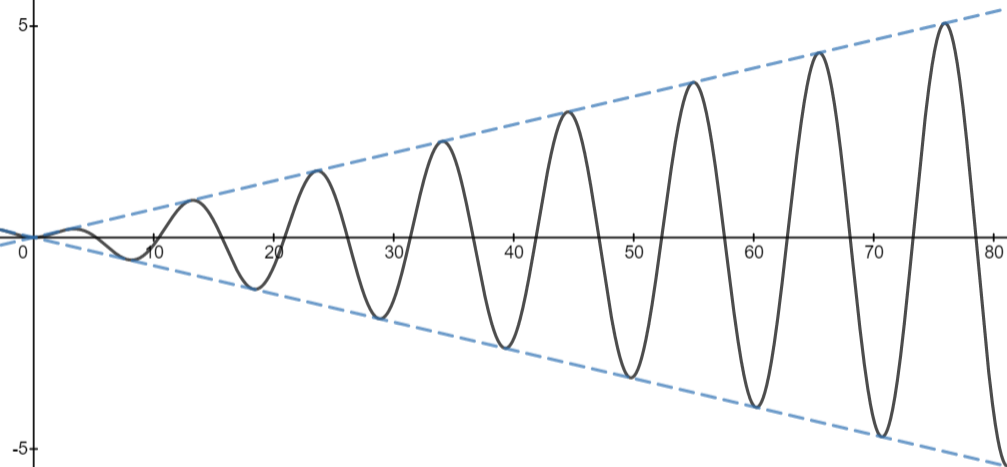
\includegraphics[width=0.75\textwidth]{./higherOrder/forcedVibrs/resonance.png}
\end{center}